\documentclass[10pt,twocolumn,letterpaper]{article}

\usepackage{cvpr}
\usepackage{times}
\usepackage{epsfig}
\usepackage{graphicx}
\usepackage{amsmath}
\usepackage{amssymb}
\usepackage[utf8]{inputenc}
\usepackage{fullpage}
\usepackage{subfig}

\usepackage[margin=1in]{geometry} 
\usepackage{amsmath,amsthm,amssymb}
 
\newcommand{\N}{\mathbb{N}}
\newcommand{\Z}{\mathbb{Z}}
 
\newenvironment{theorem}[2][Theorem]{\begin{trivlist}
\item[\hskip \labelsep {\bfseries #1}\hskip \labelsep {\bfseries #2.}]}{\end{trivlist}}
\newenvironment{lemma}[2][Lemma]{\begin{trivlist}
\item[\hskip \labelsep {\bfseries #1}\hskip \labelsep {\bfseries #2.}]}{\end{trivlist}}
\newenvironment{exercise}[2][Exercise]{\begin{trivlist}
\item[\hskip \labelsep {\bfseries #1}\hskip \labelsep {\bfseries #2.}]}{\end{trivlist}}
\newenvironment{reflection}[2][Reflection]{\begin{trivlist}
\item[\hskip \labelsep {\bfseries #1}\hskip \labelsep {\bfseries #2.}]}{\end{trivlist}}
\newenvironment{proposition}[2][Proposition]{\begin{trivlist}
\item[\hskip \labelsep {\bfseries #1}\hskip \labelsep {\bfseries #2.}]}{\end{trivlist}}
\newenvironment{corollary}[2][Corollary]{\begin{trivlist}
\item[\hskip \labelsep {\bfseries #1}\hskip \labelsep {\bfseries #2.}]}{\end{trivlist}}
 


% Include other packages here, before hyperref.

% If you comment hyperref and then uncomment it, you should delete
% egpaper.aux before re-running latex.  (Or just hit 'q' on the first latex
% run, let it finish, and you should be clear).
\usepackage[breaklinks=true,bookmarks=false]{hyperref}

\cvprfinalcopy % *** Uncomment this line for the final submission

\def\cvprPaperID{****} % *** Enter the CVPR Paper ID here
\def\httilde{\mbox{\tt\raisebox{-.5ex}{\symbol{126}}}}

% Pages are numbered in submission mode, and unnumbered in camera-ready
%\ifcvprfinal\pagestyle{empty}\fi
\setcounter{page}{1}
\begin{document}

%%%%%%%%% TITLE
\title{Textones y Clasificadores}

\author{Francisco J. Cedano\\
Departamento de Ingenier\'ia Biom\'edica\\
Universidad de Los Andes\\
{\tt\small fj.cedano803@uniandes.edu.co}
% For a paper whose authors are all at the same institution,
% omit the following lines up until the closing ``}''.
% Additional authors and addresses can be added with ``\and'',
% just like the second author.
% To save space, use either the email address or home page, not both
}%\and
%Second Author\\
%Institution2\\
%First line of institution2 address\\
%{\tt\small secondauthor@i2.org}


\maketitle
%\thispagestyle{empty}

%%%%%%%%% ABSTRACT
\begin{abstract}
   En el presente proyecto se estudia dos diferentes algoritmos para clasificar imágenes de texturas procedentes de la base de datos PONCE. Se usan dos algoritmo de clasificación. El primero es Nearest neighbour usando intersección de histogramas de textones y el segundo es Random forest. Ambos métodos se evalúan con la matriz de confusión y se estima su exactitud. Se concluye que el método Random forest tiene una exactitud del 75.6\% mientras que Nearest neighbour tiene una exactitud de 64.4\%. 
   
\end{abstract}

%%%%%%%%% BODY TEXT
\section{Introducción}

La base de datos usada en este proyecto es publicada gratuitamente por el grupo de investigación The Ponce Group de University of Illinois en Urbana-Champaigne, Estados Unidos. La base de datos consiste en 25 categorías de texturas, en cada categoría hay 40 ejemplares. Todas las imágenes están en escalas de grises, formato .jpg y tienen un tamaño de 640x480 pixels.[1]

En este proyecto se busca crear un algoritmo que permita representar diferentes imágenes por textones, posteriormente se debe diseñar dos diferentes clasificadores, entrenarlos y evaluarlos. El primer clasificador es basado en vecinos más cercanos (Nearest neighbour) y el segundo, en arboles de decisión (Random forest). Los clasificadores se evalúan con la matriz de confusión. 

%------------------------------------------------------------------------
\section{Metodología}

El primer paso para representar imágenes por textones consiste en crear el diccionario de textones. Este se hace agrupando las respuestas obtenidas de convolusionar una imagen de cada una de las 25 categorías, con un grupo de 32 filtros (Banco de Filtros). Este proceso genera datos del orden de (480 x 16000) píxeles x 32 filtros. Debido al alto costo computacional que requiere manipular estos datos, se extraen aleatoriamente 25000 textones como una muestra representativa de la población total de textones. Los textones se agruparon en 50 clusters, esto debido a que un valor pequeño de clusters no logra diferenciar textones y uno muy alto puede causar overfitting.


El filtro que más discrimina es el que tiene mayor valor de textones por filtro. Para encontrar este valor se graficó la distribución de sumas de textones por cada uno de los filtos (ver Figura 1.). Los filtros que se encontraron que tienen mayores textones son los verticales y los oblicuos (ver Figura 2.). Cabe aclarar que encontrar estos filtros requiere de estudiar el aporte global de cada filtro en cada texton. Es por ello que estos 6 filtros son los que más textones representa globalmente.

\begin{figure}[h]
\begin{center}
%\fbox{\rule{0pt}{1in} \rule{0.9\linewidth}{0pt}}
   \includegraphics[width=1\linewidth]{Filtros.png}
\end{center}
   \caption{Distribución de textones por filtro}
\label{fig:long}
\label{fig:onecol}
\end{figure}

\begin{figure}[h]
\begin{center}
%\fbox{\rule{0pt}{1in} \rule{0.9\linewidth}{0pt}}
   \includegraphics[width=1\linewidth]{FiltrosIma.png}
\end{center}
   \caption{6 Filtros más discriminadores}
\label{fig:long}
\label{fig:onecol}
\end{figure}

\begin{figure}[ht]
\centering
 \subfloat{
    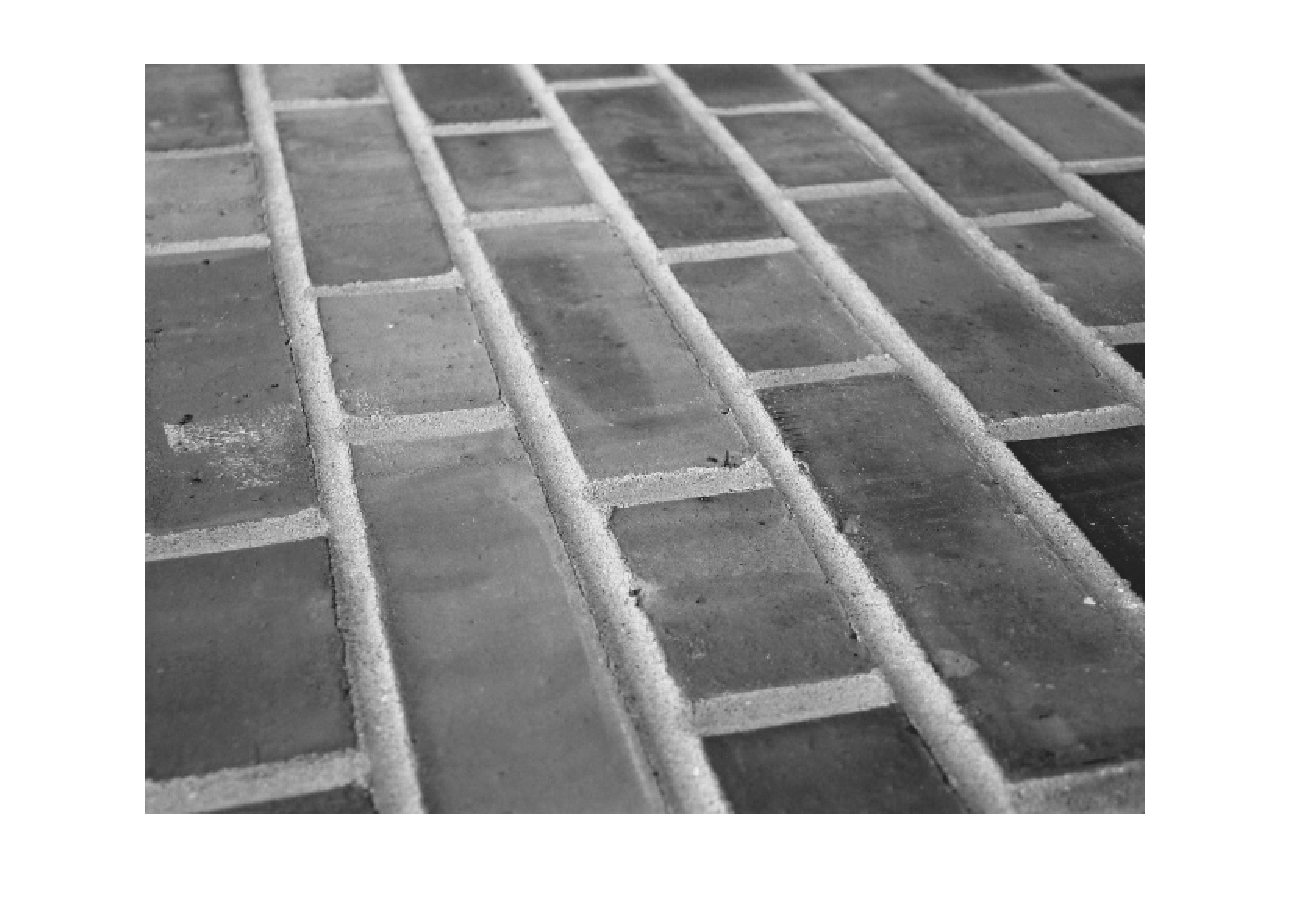
\includegraphics[width=0.5\linewidth]{Ori.eps}}
 \subfloat{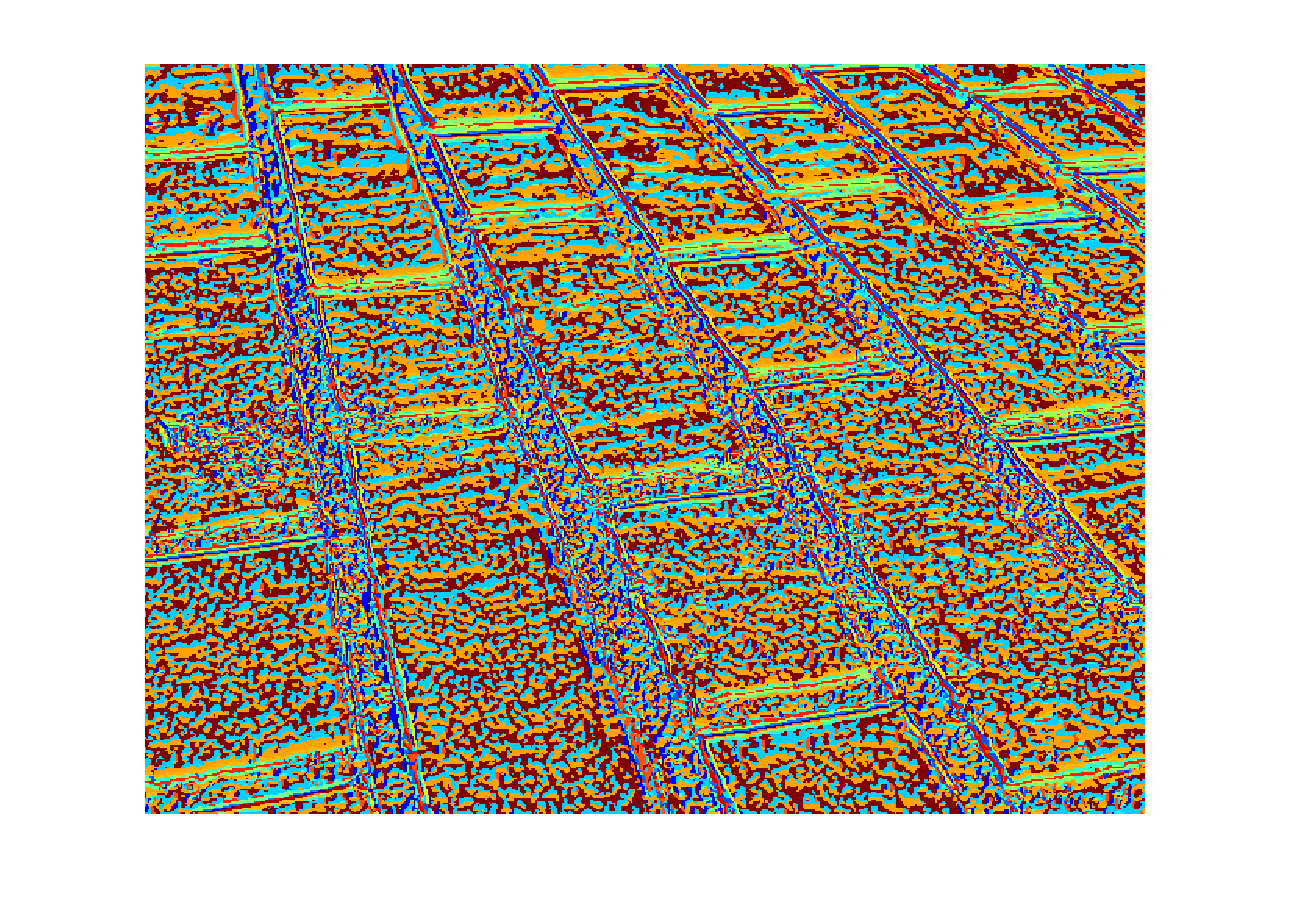
\includegraphics[width=0.5\linewidth]{Textons.eps}}
   \caption{Ejemplo de asignación de textones en una imagen de la categoría brick1, (izq.) Imagen original y (der.) mapa de textones.}
\end{figure}


\subsection{Clasificadores}

Dado un diccionario de textones, se procede a asignarlos a cada una de las imágenes de entrenamiento (750) por cada categoría (ver Figura 3.). Este proceso se hace con la función distSqr(x,y) de matlab que retorna una matriz con las distancias cuadradas entre el diccionario de textones y la nueva imagen convolusionada con el banco de filtros. (Ver Figura 4.). 


\begin{figure*}[!ht]

   \includegraphics[width=1\linewidth]{Ejemplo.png}
   \caption{(Izquierda) Imagen Original. (Centro) Mapa de Textones. (Derecha). Histograma de Textones} 
\end{figure*}

Este proceso también se hace para las imágenes de Test, debido a que se quieren comparar los histogramas de train y de test en los dos métodos de clasificación.\\

\textbf{Nearest neighbour}\\

El método de vecinos cercanos (Nearest neighbour), también conocido como interpolación próximal, es un método de interpolación multivariable en una o más dimensiones. Nearest neighbour aproxima el valor de un nuevo histograma de textones (Test), para un punto no-dado en el espacio de histogramas de textones existentes (Train). La selección de la categoría a la que pertenece la nueva imagen, va a estar dada por la mínima diferencia entre el nuevo histograma y los histogramas vecinos. Existen diversas maneras de calcular esta diferencia entre histogramas, tales como\; correlación, Chi\^2,Intersección, Bhattacharyya distance.[2] 
En este proyecto se usa el método de intersección, dado que requiere menor costo computacional que chi\^2 y es más preciso. Intersección usa el siguiente algoritmo:

\begin{align*}
\ K(a_i,b_i) & = \sum_{i=1}^{n}min(a_i,b_i)\\ 
\end{align*}

Donde a y b son dos histogramas cada uno con n bins, K es la suma de las intersecciones de los histogramas. Si se normalizan los histogramas, existirá un buen matching si K tiende a 1 y uno malo si k tiene a 0, Esto método hace más fácil la medida de similaridad.

Para calcular la intersección de los histogramas. se usó la función intersection.m del investigador B. Shauerte, publicada gratuitamente en su website [3]. Para poder usarla se debieron ajustar los histogramas de celdas a vectores con la función cell2mat de matlab. \\

\textbf{Random forest}\\

Los bosque de decisión fueron creados con la función TreeBagger de Matlab, esta función genera muestras por sobremuestreo de categorías con grandes costos de clasificación errónea y clases undersampling con pequeños costos de clasificación errónea.[4] 

Este método a diferencia de Nearest neighbour entrena un conjunto clasificación utilizando un gran conjunto de imágenes, en este caso son los histogramas de textones de entrenamiento (750) y un vector de etiquetas que identifiquen a priori la categoría a la que pertenece cada uno de los 750 histogramas.

En la etapa de entrenamiento, se construye el bosque de arboles. Para seleccionar el número de arboles, se corre la función oobError la cual permite estimar el mínimo error cuadrado para las observaciones que están fuera de clasificación de los datos de entrenamiento. Este error se grafica con respecto al número de arboles. (ver Figura 4.). A partir de este error de clasificación, se infiere que con 150 arboles el error adquiere un valor asintotico aproximadamente, y con 150 arboles es suficiente para correr la clasificación. 


\begin{figure}[h]
%\fbox{\rule{0pt}{1in} \rule{0.9\linewidth}{0pt}}
   \includegraphics[width=1\linewidth]{Errores_TreeForest.png}
   \caption{Error de clasificación en función del número de arboles}
\end{figure}

A la función TreeBagger se le añaden los siguientes parámetros.
\begin{itemize}
\item MinLeaf: Permite obtener un número mínimo de observaciones por hoja del arbol.
\item Method: Clasificación 
\end{itemize}

A partir de la construcción del arbol. Se corre los histogramas de textones de test y se usa la función Forest.predict para predecir la hoja a la que pertenecerá cada una de las nuevas imágenes. 


\subsection{Evaluación}

La evaluación de los clasificadores está dada por la matriz de confusión, la cual permite cuantificar la confusión de categorías que el método de clasificación está prediciendo. En la matriz Cada columna representa el número de predicciones de cada categoría, mientras que cada fila representa a las instancias en la categoría real.

Matlab genera la matriz de confusión con la función confusionmat en la cual le entra como parámetro las predicciones del método y las categorías reales. 

Para comparar los métodos se calcula la suma global de la diagonal de la matriz, se divide sobre el número total de imagenes de entrenamiento o de test y se multiplica por 100.

Por último se grafica las matrices de confusión de entrenamiento y de test para los resultados de los dos métodos de claificación. 
\\
\section{Resultados}

El mejor método de clasificación es el \textbf{Random forest} con un valor de 75.6\% de suma global ponderada en la diagonal de la matriz de confusión. (ver Tabla 1.)  

\begin{table}
\begin{center}
\begin{tabular}{|l|c|}
\hline
Método & Exactitud \% \\
\hline\hline
Nearest neighbour Test &  64.4\%  \\
Nearest neighbour Train &  100\% \\
Random forest Test& 75.6\% \\
Random forest Train& 92.0\% \\
\hline
\end{tabular}
\end{center}
\caption{Resultados de la suma global ponderada de las matrices de confusión para cada método en la base de datos de Train y de Test}
\end{table}

En cuanto a tiempo de entrenamiento, el método \textbf{Nearest neighbour} tiene un tiempo de cero dado que no tiene etapa de entrenamiento. Por el contrario, el método \textbf{Random forest} tiene un tiempo asociado de 626.52 segundos. Este tiempo es calculado con la función tic-toc de matlab. 

\begin{figure*}[htb]

\includegraphics[width=7in]{Matriz_Confusi_n.png}
   \caption{Matriz de confusión para el método (izq.) Nearest Neighbour y el método (der.) Random Forest. Cada matriz tiene en el eje y las categorías reales y en el eje x el número de predecciónes en esa categoría. (superior) Evaluación e (inferior) entrenamiento}
\end{figure*}

Las categorías que causan la mayor confusión  para el método de Nearest Neighbour (ver Figura 5.) son la 3, 6, 8, 20,22 y 23 (bark3, wood3, granite, fur y knit, respectivamente) con solo 5 imágenes bien clasificadas. En cambio para Random forest, las categorías de mayor confusión son 12,14,20 y 22 (brick1, glass, fur y knit, respectivamente). 

Una gran limitación de Nearest neigbour es que no tiene en cuenta información global de los histogramas de evaluación, solo tiene en cuenta información locaL con el histograma vecino más cercano.  
En cuanto a las limitaciones de random forest. Este algoritmo solo funciona bien con un número de decisiones pequeño. La selección del árbol óptimo es muy limitada y de gran dificultad. 
v Presenta inconvenientes cuando la cantidad de alternativas es grande y cuanto las decisiones no son racionales.
v Al no tener claridad de objetivos, es difícil de organizar las ideas. 

Las limitaciones de la base de datos en general son que tiene muy pocas imágenes para entrenamiento por categoría (solo 30), ademas el formato jpg no es el mejor para procesar imágenes pues se puede perder información. Pero la mayor limitación, es que las imágenes solo contienen la textura en primer plano, es decir, que una imagen de test con más información que la textura a analizar, no se podría analizar con los métodos propuestos en este proyecto.  

El método se podría mejorar añadiendo imágenes de entrenamiento más complejas y con más información ademas de la textura a analizar. 


\section{Conclusiones}

Se concluye que los 


\section{Referencias}

\begin{quote}
   
[1] S. Lazebnik, C. Schmid, and J. Ponce. A Sparse Texture Representation Using Local Affine Regions.\textit{IEEE Transactions on Pattern Analysis and Machine Intelligence} ,  pp. 1265-1278, 2005.
   
   [2] L. Clarkson, "Fast algorithms for the all nearest neighbors problem", \textit{24th IEEE Symp. Foundations of Computer Science}, pp. 226–232, 1983.
   
   [3] B. Schauerte, R. Stiefelhagen, "Learning Robust Color Name Models from Web Images". \textit{In Proceedings of the 21st International Conference on Pattern Recognition (ICPR),}, 2012
    
   [4] Matlab Documentation. TreeBagger class. mathworks.com.
   
\end{quote}

{\small
\bibliographystyle{ieee}
\bibliography{egbib}
}
\section{Anexos}
Los códigos empleados en este proyecto se adjuntan como anexo.
\begin{enumerate}
\item FJCS.m : Código para crear el diccionario de textones, de asignar los textones a cada imagen de test y de train y de construir los histogramas para cada imagen.
\item Clasificadores.m : Algoritmo de Nearest neighbour y Random forest explicado en la metodología.
\item Intersection.m : Método propuesto por [3] para comparar histogramas por intersección. 

\end{enumerate}


\end{document}
